% THIS IS SIGPROC-SP.TEX - VERSION 3.1
% WORKS WITH V3.2SP OF ACM_PROC_ARTICLE-SP.CLS
% APRIL 2009
%
% It is an example file showing how to use the 'acm_proc_article-sp.cls' V3.2SP
% LaTeX2e document class file for Conference Proceedings submissions.
% ----------------------------------------------------------------------------------------------------------------
% This .tex file (and associated .cls V3.2SP) *DOES NOT* produce:
%       1) The Permission Statement
%       2) The Conference (location) Info information
%       3) The Copyright Line with ACM data
%       4) Page numbering
% ---------------------------------------------------------------------------------------------------------------
% It is an example which *does* use the .bib file (from which the .bbl file
% is produced).
% REMEMBER HOWEVER: After having produced the .bbl file,
% and prior to final submission,
% you need to 'insert'  your .bbl file into your source .tex file so as to provide
% ONE 'self-contained' source file.
%
% Questions regarding SIGS should be sent to
% Adrienne Griscti ---> griscti@acm.org
%
% Questions/suggestions regarding the guidelines, .tex and .cls files, etc. to
% Gerald Murray ---> murray@hq.acm.org
%
% For tracking purposes - this is V3.1SP - APRIL 2009


\documentclass{sig-alternate}

\usepackage[lined,ruled,commentsnumbered,linesnumbered]{algorithm2e}
\usepackage{epstopdf}
\pagenumbering{arabic}
\usepackage{hyperref}
\newtheorem{theorem}{Assumption}

\begin{document}

\title{Distributed File Systems: \\Hadoop Distributed File System and Google File System}
%
% You need the command \numberofauthors to handle the 'placement
% and alignment' of the authors beneath the title.
%
% For aesthetic reasons, we recommend 'three authors at a time'
% i.e. three 'name/affiliation blocks' be placed beneath the title.
%
% NOTE: You are NOT restricted in how many 'rows' of
% "name/affiliations" may appear. We just ask that you restrict
% the number of 'columns' to three.
%
% Because of the available 'opening page real-estate'
% we ask you to refrain from putting more than six authors
% (two rows with three columns) beneath the article title.
% More than six makes the first-page appear very cluttered indeed.
%
% Use the \alignauthor commands to handle the names
% and affiliations for an 'aesthetic maximum' of six authors.
% Add names, affiliations, addresses for
% the seventh etc. author(s) as the argument for the
% \additionalauthors command.
% These 'additional authors' will be output/set for you
% without further effort on your part as the last section in
% the body of your article BEFORE References or any Appendices.

\numberofauthors{2} %  in this sample file, there are a *total*
% of EIGHT authors. SIX appear on the 'first-page' (for formatting
% reasons) and the remaining two appear in the \additionalauthors section.
%
\author{
% You can go ahead and credit any number of authors here,
% e.g. one 'row of three' or two rows (consisting of one row of three
% and a second row of one, two or three).
%
% The command \alignauthor (no curly braces needed) should
% precede each author name, affiliation/snail-mail address and
% e-mail address. Additionally, tag each line of
% affiliation/address with \affaddr, and tag the
% e-mail address with \email.
%
% 1st. author
\alignauthor
Ciprian Lucaci\\
       \email{ciprian.lucaci@tum.de}\\
 	 \affaddr{Technische Universit{\"a}t M{\"u}nchen, Germany}
% 2nd. author
\alignauthor
Daniel Straub\\
       \email{daniel.straub@tum.de}\\
 	 \affaddr{Technische Universit{\"a}t M{\"u}nchen, Germany}
}
% There's nothing stopping you putting the seventh, eighth, etc.
% author on the opening page (as the 'third row') but we ask,
% for aesthetic reasons that you place these 'additional authors'
% in the \additional authors block, viz.

% Just remember to make sure that the TOTAL number of authors
% is the number that will appear on the first page PLUS the
% number that will appear in the \additionalauthors section.

\maketitle
\begin{abstract}
Distributed file systems have been a technology enabler to store and process large files which exceed the size of any drive. They also work in a distributed and fail tolerant manner. The first and most known implementations are Google File System and Hadoop Distributed File System.
\end{abstract}

% A category with the (minimum) three required fields

%A category including the fourth, optional field follows...

\keywords{Distributed File Systems, Distributed Systems} % NOT required for Proceedings

%===========================================
% INTRODUCTION
\section{Introduction}
During the late 90s the Y2K issue was a popular topic in media, but together with the 2000s a bigger and more silent issue took its place. 
The rise of internet traffic, saving and processing every online footprint, having countless of sensors pouring out data into databases and then the rise of the smartphone to a omnipresence status meant that thousands of terabytes and petabytes of data were being generated daily. 
This became a problem due to multiple reasons. Firstly, there was no big enough storage medium to store all the data in a single physical location, and secondly processing such amount of data in order to extract valuable information became an even bigger challenge. Even if there were enough space to store huge amounts of data on a single drive, only seeking through such amount of data would be prohibitive in terms of access times. In this context a new IT domain was born - Big Data. 


The requirements 

Store very large data sets reliably
High bandwidth streaming
Distribute storage
Distribute computation
Analysis and transformation of data

The solution
Moving computation where data resides
Low costs - commodity machines
Vertical and Horizontal scalability

Google File System

Hadoop Distributed File System

\begin{figure}
\centering
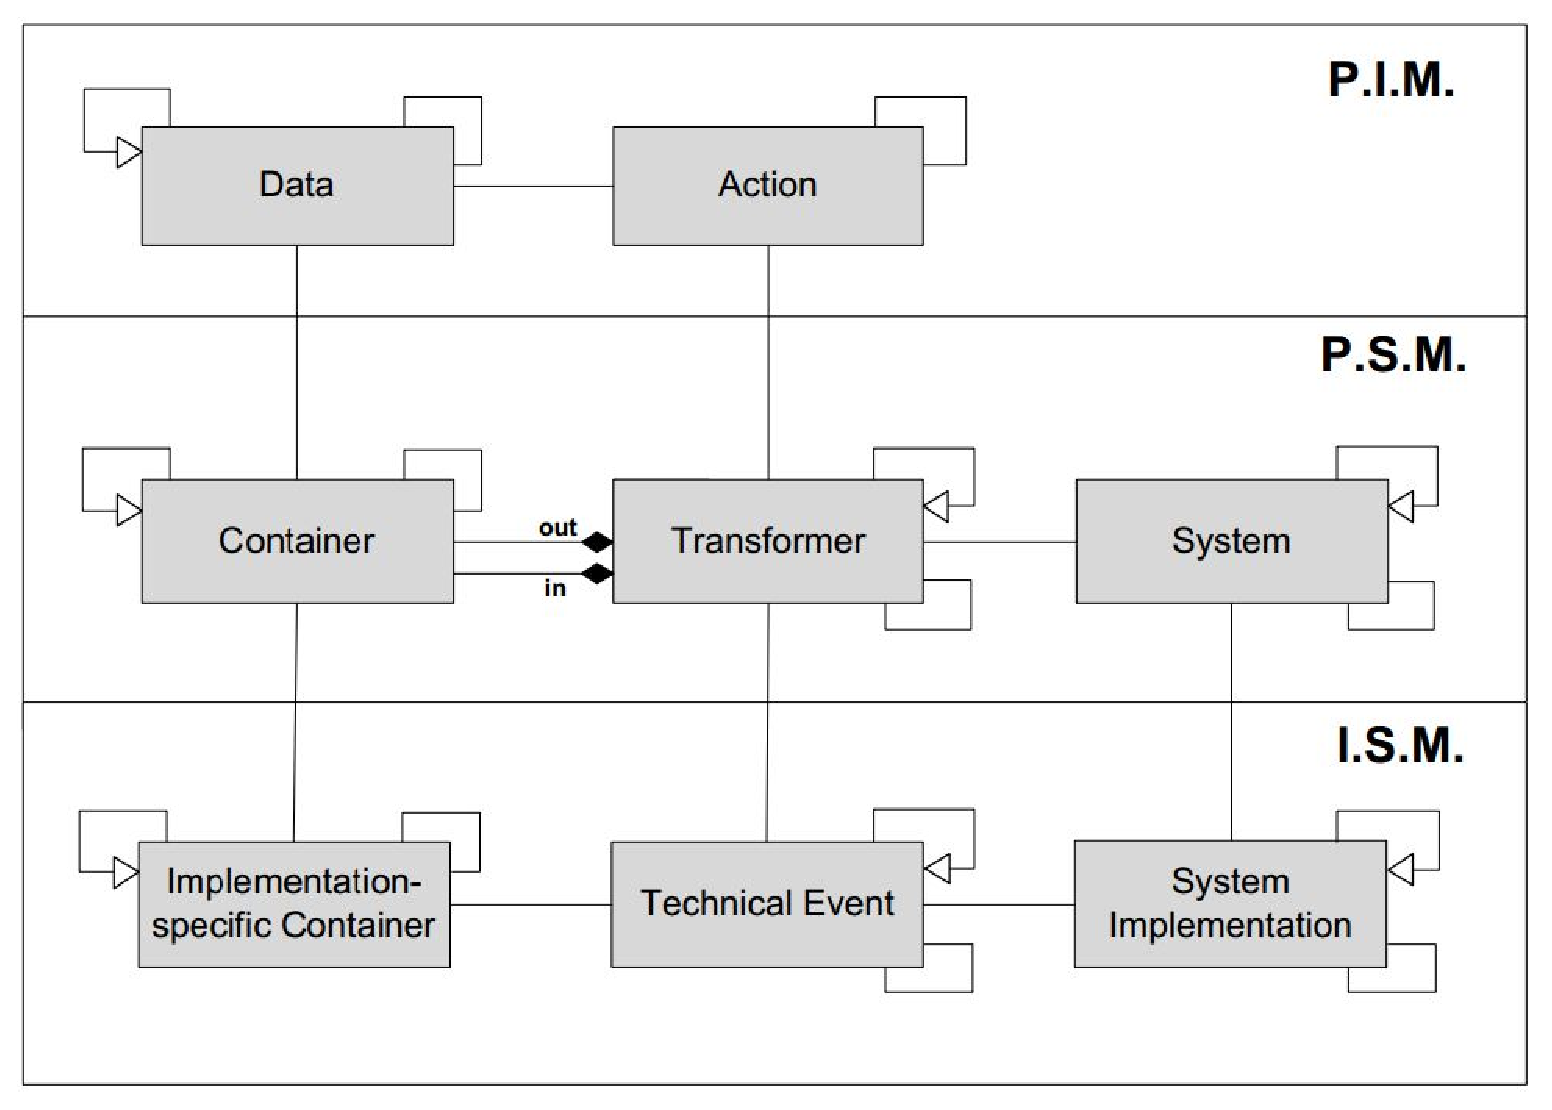
\epsfig{file=domain-meta-model.eps, height=2in, width=3in}
\caption{Domain meta-model}
\label{fig:metamodel}
\end{figure}


%===========================================
% Hadoop
\section{Hadoop Distributed File System (HDFS)}
.. add text cite~\cite{hadoop1}

Hadoop Ecosystem

\subsection{Architecture}
.. add text
\subsubsection{Blocks}
.. add text
\subsubsection{Data Nodes}
.. add text
\subsubsection{Name Node}
master-worker pattern
namespace
Inode
Metadata
Where is the namespace located

\subsubsection{Client}
.. add text
\subsubsection{Secondary Node}
- insert picture
Is there any weakness in the architecture
.. add text
Checkpoint node
Backup node

\subsection{Workflow}
.. add text
\subsubsection{Startup}
\subsubsection{Write}
.. add text code sample
\subsubsection{Read}
.. add text code sample

\subsection{Features}
.. add text
\subsubsection{Block placement policy}
\subsubsection{Replica management}
\subsubsection{Balancer}
\subsubsection{Block scanner}

\subsection{Purpose}
.. add text
Optimized for
- large files
- commodity hardware
- streaming
- batch processing
- multiple reads
Not optimized for
- big amount of small files
- concurrent modification
- arbitrary modification
- general purpose applications
Cross platform
- java, thrift, rest
- web access, console
- opensource
Companies using hdfs
- linkedin, amazon, new york times, twitter, ebay, facebook, spotify, ibm, yahoo


%===========================================
% GFS
\section{Google File System (GFS)}
.. add text
\subsection{Purpose}
.. add text
\subsection{Architecture}
.. add text
\subsection{Workflow}
.. add text
\subsection{Features}
.. add text
%===========================================
\section{Comparison}
.. add text

%===========================================
% CONCLUSIONS
\section{Conclusions and Future Work}
... not finished ...

This paragraph will end the body of this sample document.
Remember that you might still have Acknowledgments or
Appendices; brief samples of these
follow.


%\end{document}  % This is where a 'short' article might terminate


%
% The following two commands are all you need in the
% initial runs of your .tex file to
% produce the bibliography for the citations in your paper.
%===========================================
%BIBLIOGRAPHY
\bibliographystyle{abbrv}

\begin{thebibliography}{4}

\bibitem{hadoop1} Shvachko, K. and Hairong Kuang and Radia, S. and Chansler, R.: The Hadoop Distributed File System, in
\textit{Mass Storage Systems and Technologies (MSST), 2010 IEEE 26th Symposium}, pp.1-10

\bibitem{hadoop2} Hadoop: What it is and why it matters, online at
\url{http://www.sas.com/en_us/insights/big-data/hadoop.html}, [accessed: May 2015]

\bibitem{hadoop3} Hadoop tutorial, online at
\url{http://www.bigdataplanet.info/2013/10/hadoop-tutorials-part-1-what-is-hadoop.html}, [accessed: May 2015]

\bibitem{hadoop4} Thomas Kiencke: Hadoop Distributed File System,
\textit{Institute of Telematics, University of Lubeck, Germany},
 online at
\url{https://media.itm.uni-luebeck.de/teaching/ws2012/sem-sse/thomas-kiencke-hdfs-ausarbeitung.pdf}, [accessed: May 2015]

\bibitem{comparison1} R.Vijayakumari, R.Kirankumar, K.Gangadhara Rao: Comparative analysis of Google File System and Hadoop Distributed File System, in \textit{International Journal of Advanced Trends in Computer Science and Engineering}, Vol.3 , No.1, pp.: 553-558, 2014

\bibitem{google1} Sanjay Ghemawat, Howard Gobioff, and Shun-Tak Leung: The Google File System, in
\textit{Proceedings of the Nineteenth ACM Symposium on Operating Systems Principles, 2003}, pp.29-43

\end{thebibliography}  

%\balancecolumns

\balancecolumns
% That's all folks!
\end{document}
